% =====================================================================
% ELMED219: Evaluering av ML-modeller (E01-E10)
% Beamer-presentasjon i widescreen (16:9)
% =====================================================================
\documentclass[aspectratio=169, 10pt]{beamer}

% =====================================================================
% PAKKER
% =====================================================================
\usepackage[utf8]{inputenc}
\usepackage[T1]{fontenc}
\usepackage[norsk]{babel}
\usepackage{graphicx}
\usepackage{tikz}
\usepackage{booktabs}
\usepackage{amsmath}
\usepackage{fontawesome5}
\usepackage{hyperref}
\hypersetup{colorlinks=true, linkcolor=blue, urlcolor=blue}

% =====================================================================
% TEMA OG FARGER
% =====================================================================
\usetheme{Madrid}
\usecolortheme{beaver}

% Farger for TikZ-diagrammer
\definecolor{uibblue}{RGB}{0, 61, 115}
\definecolor{uibred}{RGB}{175, 28, 44}

% =====================================================================
% TITTELINFO
% =====================================================================
\title{Evaluering av ML-modeller}
\subtitle{ELMED219: Momentliste E01--E10}
\author{ELMED219}
\date{Vår 2026}

% =====================================================================
% DOKUMENT
% =====================================================================
\begin{document}

% ---------------------------------------------------------------------
\begin{frame}
    \titlepage
\end{frame}

% ---------------------------------------------------------------------
\begin{frame}{Oversikt}
    \begin{enumerate}
        \item \textbf{Confusion Matrix} (forvirringsmatrise)
        \begin{itemize}
            \item E01--E02: TP, TN, FP, FN
        \end{itemize}
        \item \textbf{Grunnleggende metrikker}
        \begin{itemize}
            \item E03: Accuracy (nøyaktighet)
            \item E04: Precision (presisjon)
            \item E05: Recall / Sensitivity (sensitivitet)
            \item E06: Specificity (spesifisitet)
        \end{itemize}
        \item \textbf{Avanserte metrikker}
        \begin{itemize}
            \item E07: F1-score
            \item E08: ROC-kurven og AUC
            \item E09: Ubalanserte datasett
            \item E10: TRIPOD-retningslinjer
        \end{itemize}
    \end{enumerate}
\end{frame}

% =====================================================================
\section{Confusion Matrix (forvirringsmatrise)}
% =====================================================================

% ---------------------------------------------------------------------
% E01
% ---------------------------------------------------------------------
\begin{frame}{E01: Tolke en Confusion Matrix (forvirringsmatrise)}

    \begin{columns}
        \begin{column}{0.45\textwidth}
            \begin{block}{Hva er det?}
                Tabell: predikerte vs. faktiske klasser
            \end{block}

            \vspace{2mm}

            \begin{center}
                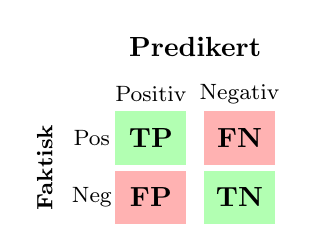
\begin{tikzpicture}[scale=0.75]
                    % Headers
                    \node at (2.25, 3.3) {\textbf{Predikert}};
                    \node at (1.5, 2.5) {\footnotesize Positiv};
                    \node at (3, 2.5) {\footnotesize Negativ};
                    \node[rotate=90] at (-0.3, 1.25) {\footnotesize\textbf{Faktisk}};
                    \node at (0.5, 1.75) {\footnotesize Pos};
                    \node at (0.5, 0.75) {\footnotesize Neg};

                    % Boxes
                    \fill[green!30] (0.9,1.3) rectangle (2.1,2.2);
                    \fill[red!30] (2.4,1.3) rectangle (3.6,2.2);
                    \fill[red!30] (0.9,0.3) rectangle (2.1,1.2);
                    \fill[green!30] (2.4,0.3) rectangle (3.6,1.2);

                    \node at (1.5, 1.75) {\textbf{TP}};
                    \node at (3, 1.75) {\textbf{FN}};
                    \node at (1.5, 0.75) {\textbf{FP}};
                    \node at (3, 0.75) {\textbf{TN}};
                \end{tikzpicture}
            \end{center}
        \end{column}
        
        \begin{column}{0.5\textwidth}
            \textbf{Avlesning:}
            \begin{itemize}
                \item \textcolor{green!50!black}{\textbf{TP}}: Korrekt positiv
                \item \textcolor{green!50!black}{\textbf{TN}}: Korrekt negativ
                \item \textcolor{red}{\textbf{FP}}: Falsk alarm
                \item \textcolor{red}{\textbf{FN}}: Oversett tilfelle
            \end{itemize}
            
            \vspace{3mm}
            
            \textbf{Eksempel:} Kreftscreening
            \begin{itemize}
                \item TP = Kreft oppdaget korrekt
                \item FN = Oversett kreft (\textit{farlig!})
            \end{itemize}
        \end{column}
    \end{columns}
    
\end{frame}

% ---------------------------------------------------------------------
% E02
% ---------------------------------------------------------------------
\begin{frame}{E02: TP, TN, FP, FN i medisinsk kontekst}
    
    \begin{table}
        \centering
        \begin{tabular}{@{}lp{5cm}p{5cm}@{}}
            \toprule
            \textbf{Term} & \textbf{Definisjon} & \textbf{Medisinsk eksempel} \\
            \midrule
            \textbf{TP} & Syk pasient, modell sier syk & Kreft korrekt identifisert \\
            \textbf{TN} & Frisk pasient, modell sier frisk & Frisk person bekreftet frisk \\
            \textbf{FP} & Frisk pasient, modell sier syk & Unødvendig biopsi \\
            \textbf{FN} & Syk pasient, modell sier frisk & \textcolor{uibred}{Oversett kreft} \\
            \bottomrule
        \end{tabular}
    \end{table}
    
    \vspace{5mm}
    
    \begin{alertblock}{Kritisk spørsmål i medisin}
        Hva er verst: \textbf{Falsk positiv} (FP) eller \textbf{Falsk negativ} (FN)?
        \begin{itemize}
            \item Screening: FN er farligere (oversett sykdom)
            \item Invasiv behandling: FP kan være farligere (unødvendig risiko)
        \end{itemize}
    \end{alertblock}
    
\end{frame}

% =====================================================================
\section{Grunnleggende metrikker (Accuracy, Precision, Recall, Specificity)}
% =====================================================================

% ---------------------------------------------------------------------
% E03
% ---------------------------------------------------------------------
\begin{frame}{E03: Accuracy (nøyaktighet)}

    \begin{block}{Definisjon}
        \[
        \text{Accuracy} = \frac{TP + TN}{TP + TN + FP + FN} = \frac{\text{Korrekte prediksjoner}}{\text{Alle prediksjoner}}
        \]
    \end{block}

    \vspace{1mm}

    \begin{columns}[T]
        \begin{column}{0.35\textwidth}
            \textbf{Eksempel:}
            \begin{center}
                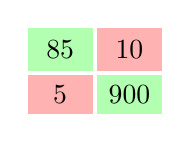
\begin{tikzpicture}[scale=0.55]
                    \fill[green!30] (0,1) rectangle (1.5,2); \node at (0.75, 1.5) {85};
                    \fill[red!30] (1.6,1) rectangle (3.1,2); \node at (2.35, 1.5) {10};
                    \fill[red!30] (0,0) rectangle (1.5,0.9); \node at (0.75, 0.45) {5};
                    \fill[green!30] (1.6,0) rectangle (3.1,0.9); \node at (2.35, 0.45) {900};
                \end{tikzpicture}
            \end{center}
        \end{column}
        \begin{column}{0.6\textwidth}
            \[
            \text{Accuracy} = \frac{85 + 900}{85 + 900 + 10 + 5} = \frac{985}{1000} = 98.5\%
            \]
        \end{column}
    \end{columns}

    \vspace{2mm}

    \begin{alertblock}{Advarsel}
        Høy accuracy kan være misvisende ved ubalanserte datasett!
    \end{alertblock}

\end{frame}

% ---------------------------------------------------------------------
% E04
% ---------------------------------------------------------------------
\begin{frame}{E04: Precision (presisjon / PPV)}
    
    \begin{block}{Definisjon}
        \[
        \text{Precision} = \frac{TP}{TP + FP} = \frac{\text{Sanne positive}}{\text{Alle predikerte positive}}
        \]
    \end{block}
    
    \vspace{3mm}
    
    \textbf{Spørsmål:} ``Av alle modellen sier er positive, hvor mange er faktisk positive?''
    
    \vspace{3mm}
    
    \begin{columns}
        \begin{column}{0.5\textwidth}
            \textbf{Høy precision viktig når:}
            \begin{itemize}
                \item Kostbar oppfølging av positive
                \item Vil unngå falske alarmer
                \item Eksempel: Sjelden sykdom
            \end{itemize}
        \end{column}
        
        \begin{column}{0.45\textwidth}
            \textbf{Eksempel:}
            \[
            \text{Precision} = \frac{85}{85 + 5} = 94.4\%
            \]
            \footnotesize\textit{``94\% av flaggede pasienter er faktisk syke''}
        \end{column}
    \end{columns}
    
\end{frame}

% ---------------------------------------------------------------------
% E05
% ---------------------------------------------------------------------
\begin{frame}{E05: Recall / Sensitivity (sensitivitet)}
    
    \begin{block}{Definisjon}
        \[
        \text{Recall} = \frac{TP}{TP + FN} = \frac{\text{Sanne positive}}{\text{Alle faktisk positive}}
        \]
    \end{block}
    
    \vspace{3mm}
    
    \textbf{Spørsmål:} ``Av alle som faktisk er positive, hvor mange fanger modellen opp?''
    
    \vspace{3mm}
    
    \begin{columns}
        \begin{column}{0.5\textwidth}
            \textbf{Høy recall viktig når:}
            \begin{itemize}
                \item Alvorlig konsekvens av å overse (FN)
                \item Screening for farlig sykdom
                \item Eksempel: Kreftscreening
            \end{itemize}
        \end{column}
        
        \begin{column}{0.45\textwidth}
            \textbf{Eksempel:}
            \[
            \text{Recall} = \frac{85}{85 + 10} = 89.5\%
            \]
            \textit{``Vi fanger opp 89.5\% av alle krefttilfeller''}
        \end{column}
    \end{columns}
    
    \vspace{2mm}

    \begin{block}{\footnotesize Andre navn}
        \footnotesize Recall = Sensitivity = True Positive Rate (TPR)
    \end{block}

\end{frame}

% ---------------------------------------------------------------------
% E06
% ---------------------------------------------------------------------
\begin{frame}{E06: Specificity (spesifisitet)}
    
    \begin{block}{Definisjon}
        \[
        \text{Specificity} = \frac{TN}{TN + FP} = \frac{\text{Sanne negative}}{\text{Alle faktisk negative}}
        \]
    \end{block}
    
    \vspace{3mm}
    
    \textbf{Spørsmål:} ``Av alle som faktisk er negative, hvor mange identifiserer modellen korrekt?''
    
    \vspace{3mm}
    
    \begin{columns}
        \begin{column}{0.5\textwidth}
            \textbf{Høy specificity viktig når:}
            \begin{itemize}
                \item Vil unngå unødvendige inngrep
                \item Kostbar/risikabel behandling
                \item Eksempel: Bekreftelsetester
            \end{itemize}
        \end{column}
        
        \begin{column}{0.45\textwidth}
            \textbf{Eksempel:}
            \[
            \text{Specificity} = \frac{900}{900 + 5} = 99.4\%
            \]
            \textit{``99.4\% av friske korrekt identifisert som friske''}
        \end{column}
    \end{columns}
    
    \vspace{2mm}

    \begin{alertblock}{\footnotesize Trade-off}
        \footnotesize Høy sensitivity $\leftrightarrow$ Lav specificity (og omvendt). Justering av terskelverdi påvirker begge.
    \end{alertblock}

\end{frame}

% =====================================================================
\section{Avanserte metrikker (F1-score, ROC/AUC, TRIPOD)}
% =====================================================================

% ---------------------------------------------------------------------
% E07
% ---------------------------------------------------------------------
\begin{frame}{E07: F1-score}
    
    \begin{block}{Definisjon}
        \[
        F1 = 2 \cdot \frac{\text{Precision} \cdot \text{Recall}}{\text{Precision} + \text{Recall}}
        \]
        \textit{Harmonisk gjennomsnitt av precision og recall}
    \end{block}
    
    \vspace{3mm}
    
    \textbf{Hvorfor harmonisk gjennomsnitt?}
    \begin{itemize}
        \item Straffer ekstreme verdier hardere enn aritmetisk gjennomsnitt
        \item Precision = 100\%, Recall = 0\% $\rightarrow$ F1 = 0\% (ikke 50\%!)
    \end{itemize}
    
    \vspace{3mm}
    
    \begin{columns}
        \begin{column}{0.48\textwidth}
            \textbf{Når bruke F1?}
            \begin{itemize}
                \item Ubalanserte datasett
                \item Når både FP og FN er viktige
                \item Sammenligne modeller
            \end{itemize}
        \end{column}
        
        \begin{column}{0.48\textwidth}
            \textbf{Eksempel:}
            \[
            F1 = 2 \cdot \frac{0.944 \cdot 0.895}{0.944 + 0.895} = 0.92
            \]
        \end{column}
    \end{columns}
    
\end{frame}

% ---------------------------------------------------------------------
% E08
% ---------------------------------------------------------------------
\begin{frame}{E08: ROC-kurven og AUC}
    
    \begin{columns}
        \begin{column}{0.45\textwidth}
            \textbf{ROC-kurve:}
            \begin{itemize}
                \item \textbf{R}eceiver \textbf{O}perating \textbf{C}haracteristic
                \item Plotter TPR vs. FPR for ulike terskler
                \item Viser trade-off mellom sensitivity og specificity
            \end{itemize}
            
            \vspace{3mm}
            
            \textbf{AUC (Area Under Curve):}
            \begin{itemize}
                \item Arealet under ROC-kurven
                \item Verdi mellom 0 og 1
                \item AUC = 0.5: tilfeldig gjetting
                \item AUC = 1.0: perfekt klassifikator
            \end{itemize}
        \end{column}
        
        \begin{column}{0.5\textwidth}
            \begin{center}
                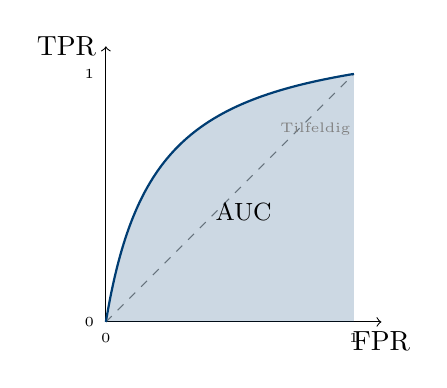
\begin{tikzpicture}[scale=0.7]
                    \draw[->] (0,0) -- (5,0) node[below] {FPR};
                    \draw[->] (0,0) -- (0,5) node[left] {TPR};
                    
                    % Diagonal (random)
                    \draw[dashed, gray] (0,0) -- (4.5,4.5);
                    
                    % Good ROC curve
                    \draw[uibblue, thick] (0,0) .. controls (0.5,3) and (1.5,4) .. (4.5,4.5);
                    
                    % Fill area
                    \fill[uibblue, opacity=0.2] (0,0) .. controls (0.5,3) and (1.5,4) .. (4.5,4.5) -- (4.5,0) -- cycle;
                    
                    \node at (2.5, 2) {\small AUC};
                    \node[gray] at (3.8, 3.5) {\tiny Tilfeldig};
                    
                    % Axis labels
                    \node at (0, -0.3) {\tiny 0};
                    \node at (4.5, -0.3) {\tiny 1};
                    \node at (-0.3, 0) {\tiny 0};
                    \node at (-0.3, 4.5) {\tiny 1};
                \end{tikzpicture}
            \end{center}
        \end{column}
    \end{columns}
    
    \vspace{3mm}
    
    \begin{block}{Tommelfingerregel}
        AUC $>$ 0.9: Utmerket \quad AUC 0.8--0.9: God \quad AUC 0.7--0.8: OK \quad AUC $<$ 0.7: Svak
    \end{block}
    
\end{frame}

% ---------------------------------------------------------------------
% E09
% ---------------------------------------------------------------------
\begin{frame}{E09: Når accuracy er utilstrekkelig}
    
    \textbf{Problemet med ubalanserte datasett:}
    
    \vspace{3mm}
    
    \begin{columns}
        \begin{column}{0.5\textwidth}
            \textbf{Eksempel:} 1000 pasienter
            \begin{itemize}
                \item 950 friske, 50 syke
                \item Modell predikerer ALLE som friske
            \end{itemize}
            
            \vspace{3mm}
            
            \textbf{Resultater:}
            \[
            \text{Accuracy} = \frac{950}{1000} = 95\%
            \]
            \[
            \text{Recall} = \frac{0}{50} = 0\%
            \]
            
            \textbf{Høy accuracy, men ubrukelig modell!}
        \end{column}
        
        \begin{column}{0.45\textwidth}
            \textbf{Løsninger:}
            \begin{itemize}
                \item Bruk F1-score eller AUC
                \item Fokuser på recall for screening
                \item Rapporter alle metrikker
                \item Sammenlign med baseline
            \end{itemize}
            
            \vspace{3mm}
            
            \textbf{Teknikker for ubalanse:}
            \begin{itemize}
                \item Oversampling (SMOTE)
                \item Undersampling
                \item Class weights
                \item Stratifisert splitting
            \end{itemize}
        \end{column}
    \end{columns}
    
\end{frame}

% ---------------------------------------------------------------------
% E10
% ---------------------------------------------------------------------
\begin{frame}{E10: \href{https://www.tripod-statement.org/}{TRIPOD}-retningslinjer}

    \begin{block}{Hva er TRIPOD?}
        \textbf{T}ransparent \textbf{R}eporting of a multivariable prediction model for \textbf{I}ndividual \textbf{P}rognosis \textbf{O}r \textbf{D}iagnosis
    \end{block}
    
    \vspace{3mm}
    
    \textbf{Hovedpunkter for rapportering av ML i medisin:}
    
    \begin{columns}
        \begin{column}{0.48\textwidth}
            \begin{enumerate}
                \item Tydelig beskrivelse av studiepopulasjon
                \item Definer utfall og prediktorer klart
                \item Beskriv missing data håndtering
                \item Rapporter modellutvikling detaljert
            \end{enumerate}
        \end{column}
        
        \begin{column}{0.48\textwidth}
            \begin{enumerate}
                \setcounter{enumi}{4}
                \item Intern validering (kryssvalidering)
                \item Ekstern validering hvis mulig
                \item Rapporter kalibrering og diskriminering
                \item Diskuter begrensninger
            \end{enumerate}
        \end{column}
    \end{columns}
    
    \vspace{5mm}
    
    \begin{alertblock}{Hvorfor viktig?}
        TRIPOD sikrer \textbf{reproduserbarhet} og \textbf{kvalitetskontroll} av prediksjonsmodeller i helseforskning.
    \end{alertblock}
    
\end{frame}

% ---------------------------------------------------------------------
% Oppsummering
% ---------------------------------------------------------------------
\begin{frame}{Oppsummering: E01--E10}

    \begin{columns}[T]
        \begin{column}{0.35\textwidth}
            \begin{center}
                \textbf{Confusion Matrix}\\[2mm]
                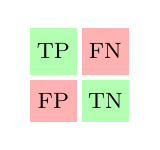
\begin{tikzpicture}[scale=0.6]
                    \fill[green!30] (0,1) rectangle (1,2); \node at (0.5, 1.5) {\footnotesize TP};
                    \fill[red!30] (1.1,1) rectangle (2.1,2); \node at (1.6, 1.5) {\footnotesize FN};
                    \fill[red!30] (0,0) rectangle (1,0.9); \node at (0.5, 0.45) {\footnotesize FP};
                    \fill[green!30] (1.1,0) rectangle (2.1,0.9); \node at (1.6, 0.45) {\footnotesize TN};
                \end{tikzpicture}
            \end{center}
        \end{column}
        \begin{column}{0.30\textwidth}
            \textbf{Metrikker:}\\[1mm]
            \footnotesize
            Recall = $\frac{\text{TP}}{\text{TP}+\text{FN}}$\\[2mm]
            Precision = $\frac{\text{TP}}{\text{TP}+\text{FP}}$\\[2mm]
            Specificity = $\frac{\text{TN}}{\text{TN}+\text{FP}}$
        \end{column}
        \begin{column}{0.30\textwidth}
            \textbf{Avansert:}\\[1mm]
            \footnotesize
            \textbf{F1-score:}\\
            Kombinerer Precision + Recall\\[2mm]
            \textbf{ROC/AUC:}\\
            Helhetsbilde uavhengig av terskel
        \end{column}
    \end{columns}

    \vspace{3mm}

    \begin{block}{\footnotesize Nøkkelpunkter}
        \footnotesize
        \begin{itemize}
            \item Velg metrikk basert på medisinsk kontekst (FN vs. FP konsekvenser)
            \item Accuracy er ofte utilstrekkelig -- bruk F1, AUC, precision, recall
            \item ROC/AUC gir helhetsbilde uavhengig av terskelverdi
            \item Følg \href{https://www.tripod-statement.org/}{TRIPOD} for transparent rapportering
        \end{itemize}
    \end{block}

\end{frame}

\end{document}








